\chapter{Introduction}\label{chapter:intro}


\section{Cosmological preliminaries}
The currently accepted cosmological model describes space-time as a 4-dimensional Lorentzian manifold equipped with the Robertson-Walker metric \cite{carroll}
\begin{equation}\label{eq_ch1:RW_metric}
    \differential s^2=c^2\differential t^2-a(t)^2\left( \frac{\differential r^2}{1-kr^2}+r^2 \differential \Omega^2 \right),
\end{equation}
with $c$ the speed of light in vacuum, $a$ the scale factor, $k$ a curvature parameter and  $\differential \Omega$ the angular volume element in spherical coordinates. The scale factor is taken to be unity at the present time. At time $t$, a physical (proper) distance $l_\text{phy}$ is then related to a comoving distance $l_\text{com}$ by 
\begin{equation}\label{eq_ch1:phy_com_dis}
    l_\text{phy}=a(t)l_\text{cov}.
\end{equation}
The physical distance at time $t$ between an observer at $r=0$ and a point at $r$ is then
\begin{equation}\label{eq_ch1:def_com_len}
    l_\text{phy}=a(t)\int_0^r \frac{\differential r}{\sqrt{1-kr^2}}=a(t)\chi(r).
\end{equation}
The Robertson-Walker metric implies that for a radial luminous signal emitted at time $t_e$ and received at time $t_0$, we have
\begin{equation}
    \differential s^2=0 \implies \frac{\differential t_0}{a(t_0)}=\frac{\differential t_e}{a(t_e)}.
\end{equation}
As a consequence, the received frequency is redshifted according to
\begin{equation}
    1+z=\frac{\lambda_0}{\lambda_e}=\frac{\nu_e}{\nu_0}=\frac{a(t_0)}{a(t_e)},
\end{equation}
where $z$ is the redshift.

The time-dependence of physical distances in \cref{eq_ch1:phy_com_dis} implies that an object whose comoving distance $\chi$ to an observer is constant recedes by following the Hubble flow according to
\begin{equation}\label{eq_ch1:hubble_law}
    v(t)=\dot{a}(t)\chi=\frac{\dot{a}}{a}a\chi=H(t)l_\text{phy},
\end{equation}
where $H(t)$ is known as the Hubble factor. \cref{eq_ch1:hubble_law} is known a Hubble's law. At present time, $H(t_0)=H_0$ is referred to as Hubble'2 constant. For historical reasons, it is common to work with the reduced Hubble constant $h=H_0 [\text{km/s/Mpc}]/100$.
Note that, according to \cref{eq_ch1:def_com_len}, and using the Robertson-Walker metric for a radial light signal, we obtain
\begin{equation}
    \differential \chi=\frac{c\differential t}{a}\implies \chi=\int_a^1\frac{\differential a}{a \dot{a}}=\int_0^z\frac{c \differential z}{H(z)}.
\end{equation}
As a consequence, the proper line element satisfies
\begin{equation}\label{eq_ch1:dl_over_dz}
    \differential \chi =\frac{c\differential z}{H(z)}=\frac{dl}{a(t)} \implies \frac{\differential l}{\differential z}=\frac{c}{(1+z)H(z)},
\end{equation}
which will be useful when integrating quantities along a line of sight. When working with such sightlines in spectroscopy, it is often advantageous to work with velocity units instead of redshifts (or proper distances). Differentiating \cref{eq_ch1:hubble_law} and considering a slow varying Hubble factor around a mean redshift $\overline{z}$, we obtain the following useful expression:
\begin{equation}
    \differential v=H(\overline{z})\differential l=H(\overline{z})\frac{c\differential z}{(1+\overline{z})H(\overline{z})}=\frac{c\differential z}{1+\overline{z}}.
\end{equation}

The evolution of the scale factor (and hence of the redshift) with time is completely determined by the energy content of the universe through Einstein's field equation, which is known as Friedmann's equation in this context
\begin{equation}
    H^2=H_0^2\left( \Omega_\text{M} (1+z)^3+\Omega_\text{R} (1+z)^3 +\Omega_\Lambda + \Omega_K (1+z)^2 \right)=H_0^2E(z)^2,
\end{equation}
where the density parameters $\Omega$ are related to the physical densities of the components according to
\begin{equation}\label{eq_ch1:density_params}
    \begin{aligned}&\Omega_\text{M}&&=\quad\frac{8\pi G}{3H_0^2}\rho_{M0}\\&\Omega_\text{R}&&=\quad\frac{8\pi G}{3H_0^2}\rho_{R0}\\&\Omega_{\Lambda}&&=\quad\frac{8\pi G}{3H_0^2}\rho_{\Lambda}\\&\Omega_\text{K}&&=\quad-\frac k{H_0^2}\end{aligned}
\end{equation}
In \cref{eq_ch1:density_params}, $\rho_\text{M}$ denotes the matter density of the universe, $\rho_\text{R}$ the radiation density, and $\rho_\Lambda$ the dark energy component. In the following, the values used for the cosmological parameters are $\Omega_m=0.308,\Omega_\Lambda=0.692,h=0.678,\Omega_b=0.0482,\sigma_8=0.829\mathrm{~and~}n=0.961, \Omega_\text{K}\approx 0$, as obtained from CMB measurements by the Planck Collaboration \cite{planck2014}. With the previous cosmological parameters, the matter and cosmological constant are equal when
\begin{equation}
    \Omega_\text{M}(1+z)^3=\Omega_\Lambda \implies z\approx 0.3.
\end{equation}
In consequence, at the redshift of interest for this work, $z\sim 4-5$, the universe is well-described as a matter dominated universe.





\section{Dark matter}
\subsection{Evidence for the inclusion of dark matter in the cosmological model}
\subsection{Manifold dark matter candidates}
\subsection{Constraining mechanisms for dark matter}



\section{The intergalactic medium}

\subsection{The Lyman-alpha forest as a probe of the IGM}

Let us now describe how an intergalactic cloud (with no peculiar velocity) along the line of sight of a quasar affects its spectrum, allowing for a powerful probing mechanism of the IGM. Consider the situation illustrated in \cref{fig_ch1:Lyman_alpha_diagram}, where a QSO at redshift $z_\text{QSO}$ emits photons, and consider the propagation of an emitted photon with rest-frame frequency $\nu_e$. Those photons are redshifted and are absorbed at $z_\alpha$ by a neutral hydrogen absorber with local number density $n(z_\alpha)$ producing an absorption feature in the flux at the rest-frame Lyman-$\alpha$ resonance $\lambda_\alpha \approx 1215$\r{A}. The unabsorbed photons are then redshifted and are detected by an observer at $z=0$ and a frequency $\nu_o$. The relationship between the frequencies mentioned above is then:
\begin{equation}
    \nu_o=\frac{\nu_e}{1+z_e}=\frac{\nu_\alpha}{1+z_\alpha} 
\end{equation}

\begin{figure}[t]
    \centering
    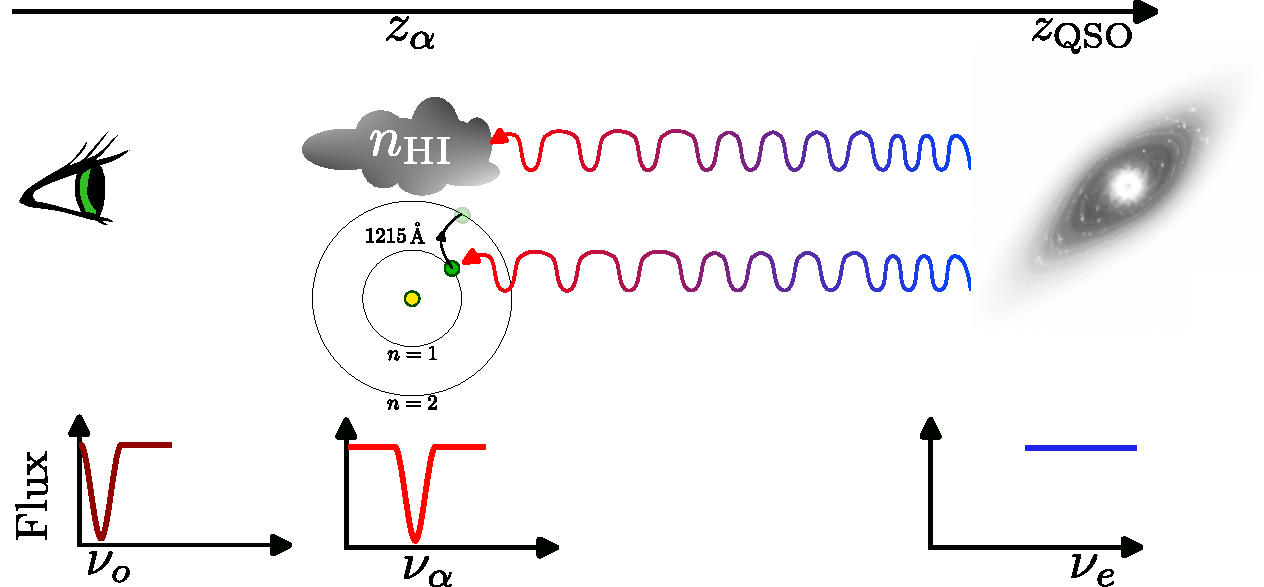
\includegraphics[width=1\linewidth]{img/lyman-alpha.pdf}
    \caption{Illustration of the Lyman-$\alpha$ absorption by neutral hydrogen at $z=z_\alpha$ in the line of sight of a QSO at $z=z_{\text{QSO}}$. In the observer's rest frame, the observed frequency is $\nu_o$. The associated frequency emitted by the QSO is $\nu_e$. }
    \label{fig_ch1:Lyman_alpha_diagram}
\end{figure}
We are interested in studying the effect of the Lyman-$\alpha$ absorbed at $z_\alpha$. The observed flux attenuation at the observed frequency $\nu_0$ is then expressed as $\exp(-\tau_\alpha)$, with $\tau_\alpha$ the Lyman-$\alpha$ opacity at the observed frequency, which depends on the observer's density and the Lyman-$\alpha$ cross-section $\sigma_\alpha(\nu)$. Observe now that since the Lyman-$\alpha$ cross-section is strongly peaked at the resonance $\nu_\alpha$, but can have a non-zero width, a nearby neutral hydrogen cloud might absorb photons at a redshift different to $z_\alpha$ that would have contributed to the observed flux at frequency $\nu_o$. With this consideration, we integrate over the line of sight to obtain the Lyman-$\alpha$ opacity at the observed frequency

\begin{equation}\label{eq_ch1:GP_integral}
    \tau_\alpha(\nu_o)=\int_o^{z_\text{QSO}} n_\text{HI}(z) \sigma_\alpha[\nu_o(1+z)] \differential z.
\end{equation}
If we now take $\sigma_\alpha(\nu)$ to be a Dirac delta centered at the resonance $\nu_\alpha$ and we integrate \cref{eq_ch1:GP_integral} by using \ref{eq_ch1:dl_over_dz} we obtain

\begin{equation}\label{eq_ch1:GP_approx}
    \tau_\alpha(\nu_o)\approx \frac{cn_\text{HI}(z_\alpha)\sigma_\alpha}{H_0\Omega_\text{m}^{1/2} (1+z)^{1/3}},
\end{equation}
where now $\sigma_\alpha=4.5 \times 10^{-18}$cm$^2$ is to total Lyman-$\alpha$ cross-section.
\cref{eq_ch1:GP_approx} is know as the Gunn-Peterson approximation for the Lyman-$\alpha$ opacity of the IGM \cite{GunnPeterson}. \cref{eq_ch1:GP_approx} demonstrates that quasar spectra are a useful probe of the intergalactic neutral hydrogen density.

The Gunn-Peterson Lyman-$\alpha$ opacity can then be used to estimate the average neutral hydrogen fraction $x_\text{HI}$. The evolution of the observed Lyman-$\alpha$ optical depth indicates that the IGM is highly ionized at $z\lessapprox 5.5$, \cite{Becker_2001_GP_trough}, \cite{Ian_model_inde_reio}.

\begin{figure}
    \centering
    \includegraphics[scale=0.7]{img/ML/villa_wdm.png}
    \caption{Baryonic density plot of the IGM as a function of redshift, and the WDM model mass. On the horizontal axis, the time evolution shows how gravity collapses dense regions into structures. On the vertical axis, the WDM free-streaming length suppress small-scale clustering. Extracted from \cite{Villasenor_2023}.}
    \label{fig:villasenor_wdm}
\end{figure}

discuss villa plot and pdf and ps plot

ADD notations about overdensityes, relatio nship with omega etc
IGM typical density, temp, temp-density relationship, UVB,phoion equiv
Gun Peterson test, and reionization constraints
contribution to UVB?
ADD IN THE INTRO SOME ABOUT GR AND METRIC
ADD SECTION 2.8.2 OF BOOk
ADD BOLTON ARTICLE WITH UVB AND INFO